\documentclass[12pt,letterpaper]{article}
\usepackage{amsmath,amsthm,amsfonts,amssymb,amscd}
\usepackage{listings}
\usepackage{color}

\definecolor{dkgreen}{rgb}{0,0.6,0}
\definecolor{gray}{rgb}{0.5,0.5,0.5}
\definecolor{mauve}{rgb}{0.58,0,0.82}

\lstset{%frame=tb,
  language=Bash,
  aboveskip=3mm,
  belowskip=3mm,
  showstringspaces=false,
  columns=flexible,
  basicstyle={\small\ttfamily},
  numbers=none,
  numberstyle=\tiny\color{gray},
  keywordstyle=\color{blue},
  commentstyle=\color{dkgreen},
  stringstyle=\color{mauve},
  breaklines=true,
  breakatwhitespace=true
  tabsize=3
}


\usepackage{hyperref}
\usepackage{graphicx}
\usepackage{enumerate}
\usepackage{fancyhdr}
\usepackage{mathrsfs}
\usepackage[margin=3cm]{geometry}
\setlength{\parindent}{0.0in}
\setlength{\parskip}{0.05in}

% Edit these as appropriate
\newcommand\course{CS595}
\newcommand\semester{FAll 2013}     
\newcommand\hwnum{3}
\newcommand\yourname{Mohamed Aturban}
\newcommand\login{maturban}

\newenvironment{answer}[1]{
  \subsubsection*{Problem #1}
}

\pagestyle{fancyplain}
\headheight 40pt
\lhead{\yourname\ (\login)\\\course\ --- \semester}
\chead{\textbf{\Large Assignment \hwnum}}
\rhead{\today}
\headsep 40pt

\begin{document}

All files mentioned in this document should be uploaded into the {\it github} repository.

\begin{answer}{1}
A shell script, called {\it ranking.sh}, is created by a Python program -- {\it ranking.py}. This script contains commands that will achieve the following tasks:
\begin{itemize}
\item Downloading the 1000 URIs from the previous assignment using curl. See examples below:
\begin{lstlisting}
	$curl www.cnn.com > file1.html
	$curl www.yahoo.com > file2.html
	$curl www.alarabiya.com > file3.html
	...
	
\end{lstlisting}

The output files will have their names with sequential numbers (e.g. {\it file1.html}, {\it file2.html}, ...,{\it file1000.html}). A number in a file name indicates a specific URL. In other words, {\it file1.html} contains the raw {\it html} format of the first URI listed in the file {\it links.txt} while {\it file2.html} is the raw {\it html} format corresponding to the second URI in {\it links.txt} and so on.

\item Remove (most) of the HTML markup from {\it .html} files and store results in files called: {\it file1.html.processed}, {\it file2.html.processed}, ..., {\it file1000.html.processed}. This can be done by the {\it lynx} command:

\begin{lstlisting}
	$lynx -dump -force_html file1.html > file1.html.processed
	$lynx -dump -force_html file2.html > file2.html.processed
	$lynx -dump -force_html file3.html > file3.html.processed
	...

\end{lstlisting}
\end{itemize}

%\begin{figure}[ht!]
%\centering
%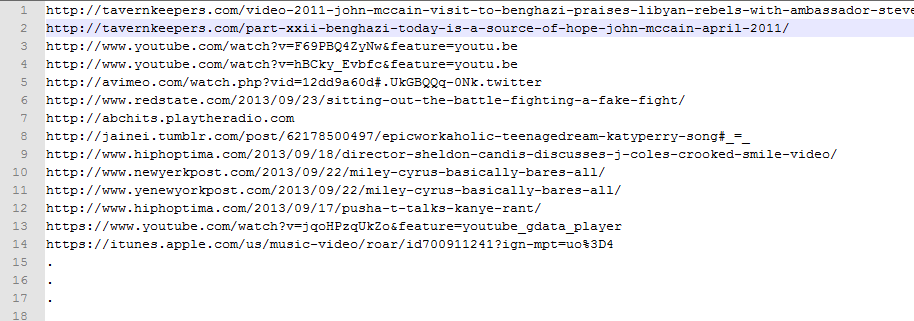
\includegraphics[scale=0.75]{links11}
%\caption{Output URIs}
%\label{overflow}
%\end{figure}
\end{answer}


\begin{answer}{2}

To count number of words, another two commands are added to the shell script {\it ranking.sh}:

\begin{itemize}
\item By {\it wc} command, a list of numbers of all words of all {\it .processed} files can be obtained. This list will be stored in a file called {\it wordsFreq.txt}. See the following examples:
\begin{lstlisting}
	$wc -w < file1.html.processed >> wordsFreq.txt
	$wc -w < file2.html.processed >> wordsFreq.txt
	$wc -w < file3.html.processed >> wordsFreq.txt
	...
\end{lstlisting}
The output of {\it wordsFreq.txt}:
\begin{lstlisting}
	1127
	2259
	1322
	...
\end{lstlisting}

\item By both {\it grep} and {\it wc} commands, we can get a list of numbers of occurrences of a term in all {\it .processes} files. In this assignment, I have chosen the term {\bf song}. The output will be stored in a file called {\it termFreq.txt}:

\begin{lstlisting}
	$grep -rohiw Shakira file1.html.processed | wc -w >> termFreq.txt
	$grep -rohiw Shakira file2.html.processed | wc -w >> termFreq.txt
	$grep -rohiw Shakira file3.html.processed | wc -w >> termFreq.txt
	...

\end{lstlisting}
The output of {\it termFreq.txt}:
\begin{lstlisting}
	0
	0
	0
	.
	.
	.
	7
	3
	...
\end{lstlisting}

\end{itemize}


Because we are to choose only 10 documents containing the term, I have done all calculations shown in the below table manually.

\begin{itemize}
\item Number of Documents = 1000
\item Number of Documents with the term song = 133
\end{itemize}

See table 1 for results.

\begin{table}[ht]
    \begin{tabular}{ |  p{1.2cm} |  p{1.2cm} | l | p{2.4cm} | l | p{8cm} |}

    \hline
    Words in Doc. & Term Freq.  & TF & IDF(song) & TFIDF & URI \\ \hline

	836 & 8 & 0.010 & 2.911 & 0.028 &  \url{http://www.youtube.com/watch?v=OFGgbT_VasI&feature=youtu.be
} \\ \hline
	809 & 6 & 0.007 & 2.911 & 0.022 &  \url{http://www.youtube.com/watch?v=2XMN2dg7OuU
} \\ \hline
	873 & 6 & 0.007 & 2.911 & 0.020 &  \url{http://www.youtube.com/watch?v=qjOeKRb6fco&feature=youtu.be
} \\ \hline
	1194 & 4 & 0.003 & 2.911 & 0.010 &  \url{https://www.youtube.com/watch?v=ln_RwnQC_vQ&feature=youtube_gdata_player
} \\ \hline
	650 & 2 & 0.003 & 2.911 & 0.009 &  \url{http://musiclikeneverbefore.com/index.html
} \\ \hline
	1059 & 3 & 0.003 & 2.911 & 0.008 &  \url{http://www.youtube.com/watch?v=c7Rd5rchoiI
} \\ \hline
	1034 & 2 & 0.002 & 2.911 & 0.006 &  \url{http://www.youtube.com/watch?v=xI44Xr2D0Ck&feature=youtu.be
} \\ \hline
	1241 & 2 & 0.002 & 2.911 & 0.005 &  \url{http://www.mjtunes.com/
} \\ \hline
	1750 & 3 & 0.002 & 2.911 & 0.005 &  \url{http://www.youtube.com/watch?v=s8QYxmpuyxg&list=PLEUun43OsA1egklY4LVnkO_Satgfy-TYO
} \\ \hline
	3825 & 4 & 0.001 & 2.911 & 0.003 & \url{http://www.5pinkave.com/} \\ \hline









    \end{tabular}
\caption{10 Hits for the term : {\bf song}}	
\end{table}
\end{answer}

\begin{answer}{3}

Table 2 shows the estimation of the page rank of the 10 URI included in table 1 using the following page rank estimator:\url{http://www.seocentro.com/tools/search-engines/pagerank.html}. Because this tool always gives a page rank between 1 and 10, the result is divided by 10 to normalize the value to be from 0 to 1. Before even starting this experience, I was almost sure that the result produced from both mechanisms will be totally different since they use different algorithms to produce the page rank. I think the page rank estimators, mentioned in question 3, involve more complicated computations. I was surprised when seeing 50 percent of the results in table 1 and 2 are identical. URIs, placed in rows 1, 3, 4, 6 and  10 are the same pages in both tables! On the other hand, I can not recognize any pattern for the rest 5 pages. For example, The URL, placed in row 2 in table 1, is in row 8 in table 2 while the fifth URL in table 1 is placed in row 9 in table 2. 


\begin{table}[ht]
    \begin{tabular}{ | p{1.8cm} |  p{13cm} | }

    \hline
    Page Rank & URI \\ \hline

0.6 & \url{http://www.youtube.com/watch?v=OFGgbT_VasI&feature=youtu.be
} \\ \hline
0.6 & \url{http://www.youtube.com/watch?v=s8QYxmpuyxg&list=PLEUun43OsA1egklY4LVnkO_Satgfy-TYO
} \\ \hline
0.5 & \url{http://www.youtube.com/watch?v=qjOeKRb6fco&feature=youtu.be
} \\ \hline
0.4 & \url{https://www.youtube.com/watch?v=ln_RwnQC_vQ&feature=youtube_gdata_player
} \\ \hline
0.4 & \url{http://www.youtube.com/watch?v=xI44Xr2D0Ck&feature=youtu.be
} \\ \hline
0.3 & \url{http://www.youtube.com/watch?v=c7Rd5rchoiI
} \\ \hline
0.3 & \url{http://www.mjtunes.com/
} \\ \hline
0.2 & \url{http://www.youtube.com/watch?v=2XMN2dg7OuU
} \\ \hline
0.2 & \url{http://musiclikeneverbefore.com/index.html
} \\ \hline
0.0 & \url{http://www.5pinkave.com/
} \\ \hline

    \end{tabular}
\caption{The page rank estimation for the 10 URIs included in table 1}	
\end{table}

\end{answer}

\begin{answer}{4}

As mentioned in `http://stackoverflow.com/questions/2557863/measures-of-association-in-r-kendalls-tau-b-and-tau-c`

$Kendall Tau_b = (P - Q) / ( (n0 - n1)(n0 - n2) ) ^{1/2} $

$ Where: $

P: concordant pairs 

Q: discordant pairs 

N0: n(n-1) / 2

n1: the number of tied pairs on x 

n2: the number of pairs pairs tied on y 

\begin{table}[ht]
    \begin{tabular}{ | p{1.8cm} | p{1.8cm} | p{6cm} | p{6cm} | }

    \hline
    TFIDF & Page Rank & Y pairs in natural order
 & Y pairs in reverse natural order
  \\ \hline

0.003 & 0.0 & 9 & 0 \\ \hline
0.005 & 0.3 & 5 & 2 \\ \hline
0.005 & 0.6 & 1 & 6 \\ \hline
0.006 & 0.4 & 3 & 3 \\ \hline
0.008 & 0.3 & 3 & 2 \\ \hline
0.009 & 0.2 & 4 & 0 \\ \hline
0.010 & 0.4 & 2 & 1 \\ \hline
0.020 & 0.5 & 1 & 1 \\ \hline
0.022 & 0.2 & 1 & 0 \\ \hline
0.028 & 0.6 & 0 & 0 \\ \hline


    \end{tabular}
\caption{ to compute P, Q, X0 and Y0 values }	
\end{table}


From table 3 when can get the following:

P = 29

Q = 15

n0 = ( 10 * 9)/2  = 45

n1 = 2(1) / 2 = 1

N2 = ( 2(1) + 2(1) + 2(1)+ 2(1) ) / 2 =4


$ Kendall Tau_b = (29 - 15) / ( (45 - 1)(45 - 4) ) ^{1/2} $

$ Kendall Tau_b =  0.32 $


$P = ((n * \sum_{i=1}^n xy) - ( sum_{i=1}^n x * sum_{i=1}^n y )) / ( \sqrt{n (sum_{i=1}^n x^2) - (sum_{i=1}^n x)^2 } * \sqrt{n (sum_{i=1}^n y^2) - (sum_{i=1}^n y)^2 }  )$

P = 0.011

\end{answer}

\end{document}
